\section{Generowanie raportu}

Docelowym działaniem aplikacji, będącym zwieńczeniem wszystkich jej funkcjonalności, jest możliwość wygenerowania finalnego raportu w formacie arkusza kalkulacyjnego na podstawie uzupełnionej bazy danych. W związku z tym w Power Apps przygotowano mechanizm łączący dane z trzech list sharepointowych, które następnie są przesyłane do Power Automate, gdzie podlegają dalszemu przetwarzaniu. Wynikiem tego jest kompletny arkusz Excel, który jest zapisywany na platformie SharePoint.

\subsection{Łączenie źródeł danych do formy docelowej}

Pierwszym krokiem do wygenerowania gotowego raportu jest konsolidacja potrzebnych danych w odpowiedniej formie. Do tego celu zaimplementowano ekran przedstawiony na rysunku \ref{fig:generateraportform}. Składa się on z dwóch formularzy -- węższy po lewej stronie oraz szerszy po prawej. W pierwszym z nich znajdują się dwa 
pola wyboru typu \emph{Dropdown}, w których należy wybrać numer indykacji oraz roku do pobrania danych z list, natomiast w drugiej widnieje podgląd zawartości danych do wygenerowania w formie tabeli, która może zostać przekazana do Power Automate.

\begin{figure}[H]
    \centering
    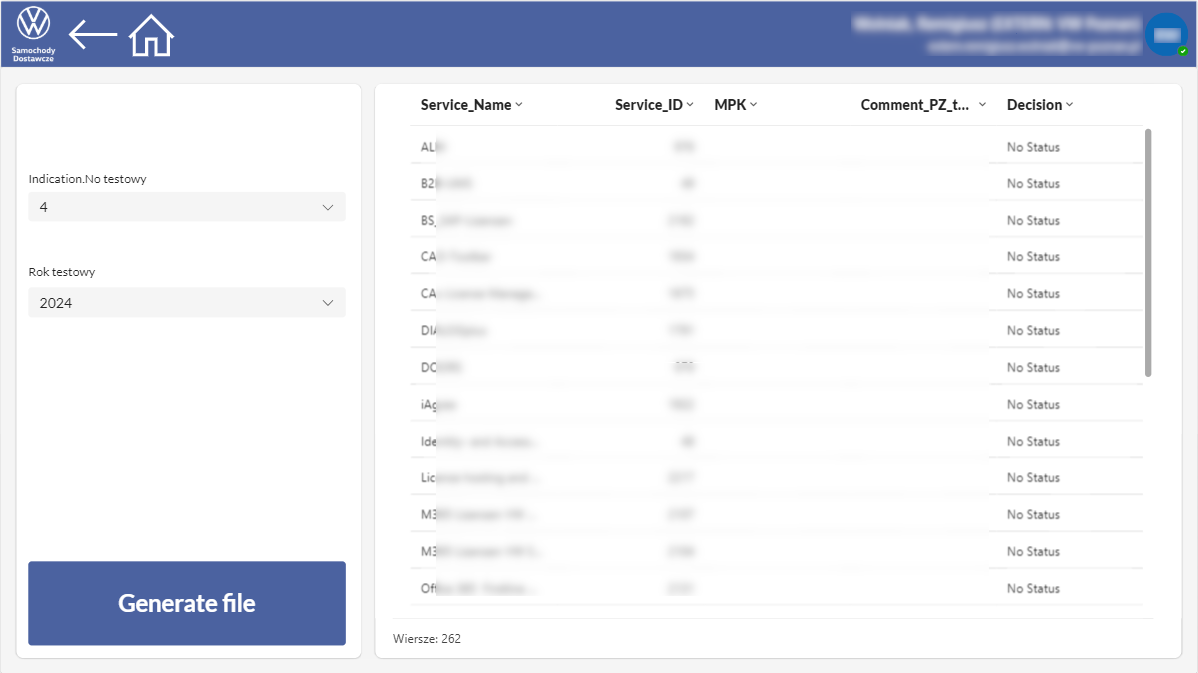
\includegraphics[width=0.9\textwidth]{figures/GenerateRaportForm.png}
    \caption{Ekran generowania raportu} 
    \label{fig:generateraportform}
\end{figure}

Zebrane dane przechowywane są w tymczasowej kolekcji \textit{CombinedData}, która składa się z informacji z trzech źródeł, odpowiednio dopasowanych do wybranego przez użytkownika roku oraz indykacji. Przykładowy fragment kodu odpowiedzialnego za tworzenie tej kolekcji przedstawiono w listingu~\ref{lst:combineddata}:

\begin{lstlisting}[language=PowerFx, caption={Fragment kodu tworzącego kolekcję CombinedData}, label={lst:combineddata}] 
    ClearCollect(
    CombinedData;
    AddColumns(
        LocalServiceData;
        MPK;
        LookUp(
            LocalCostData;
            Service_ID = LocalServiceData[@Service_ID] && Year = Year_Dropdown_1.Selected.Value;
            MPK
        );
        Comment_PZ_to_WOB;
        LookUp(
            LocalIndicationsData;
            Service_ID = LocalServiceData[@Service_ID] && Year = Year_Dropdown_1.Selected.Value && IndicationNo = IndicationNo_Dropdown_1.Selected.Value;
            Comment_PZ_to_WOB);     
    [...]
);;

\end{lstlisting}

W fragmencie kodu przedstawiono wykorzystanie funkcji \textit{LookUp}, która pozwala na pobranie danych z różnych kolekcji na podstawie określonych kryteriów. Przykładowo, pierwsze wywołanie \textit{LookUp} dopasowuje dane z tabeli \textit{LocalCostData}

\customnote{Nie no musze zobaczyc w apce jak te lookupy byly zrobione bo nie pamietam, ale to jutro. \textbf{Przecież masz w kodzie xD}}


\subsection{Przekazywanie danych do Power Automate}

W lewym dolnym rogu interfejsu znajduje się przycisk \textit{Generate file}, który po naciśnięciu uruchamia \textit{flow} w Power Automate, odpowiedzialny za tworzenie pliku na podstawie danych wejściowych. Dane te są przekazywane do usługi Power Automate w postaci ciągu tekstowego, sformatowanego jako JSON\footnote{JSON - format wymiany danych, który jest oparty na strukturze tekstowej}, wykorzystując połączone informacje z trzech źródeł zawarte w kolekcji \textit{CombinedData}, dostosowane do wybranego przez użytkownika zestawu roku i indykacji. Kod wywołujący funkcję \textit{GenerateRaport} przedstawiono w listingu~\ref{lst:generateraport}.



\begin{lstlisting}[language=PowerFx, caption={Kod wywołujący funkcję GenerateRaport}, label={lst:generateraport}]
    GenerateRaport.Run(
        Substitute(
            "[" & 
            Concat(
                CombinedData;
                "{""Service_ID"":""" & Service_ID & """," &
                """Service_Name"":""" & Service_Name & """," &
                """MPK"":""" & MPK & """," &
                """Comment_PZ_to_WOB"":""" & Comment_PZ_to_WOB & """," &
                """Decision"":""" & Decision & """},"
            ) & 
            "]",
            "},]"; 
            "}]"
        ),
        IndicationNoCollect.Value,
        YearNoCollect.Value
    )
    \end{lstlisting}

